\chapter{Project Plan}

The Project Plan of this Master's Dissertation is visualized in figure
\ref{fig:ProjectPlan}. The critical, red path is the result of the
parallelization of some work packages. These packages mostly are independent and
include idle time delays, so that it is more efficient to parallelise them. For 
example we can regard the simulation and research together with the Master's Thesis documentation. These work packages can be parallelized, because the
simulations which have to be executed are time intensive and not a basic part of
the complete documentation. Furthermore we can see that one cycle of the spiral
model will be executed in the context of this Master's Thesis including an
iteration of the \MBD process.

\begin{figure}[!htbp]
	\centering
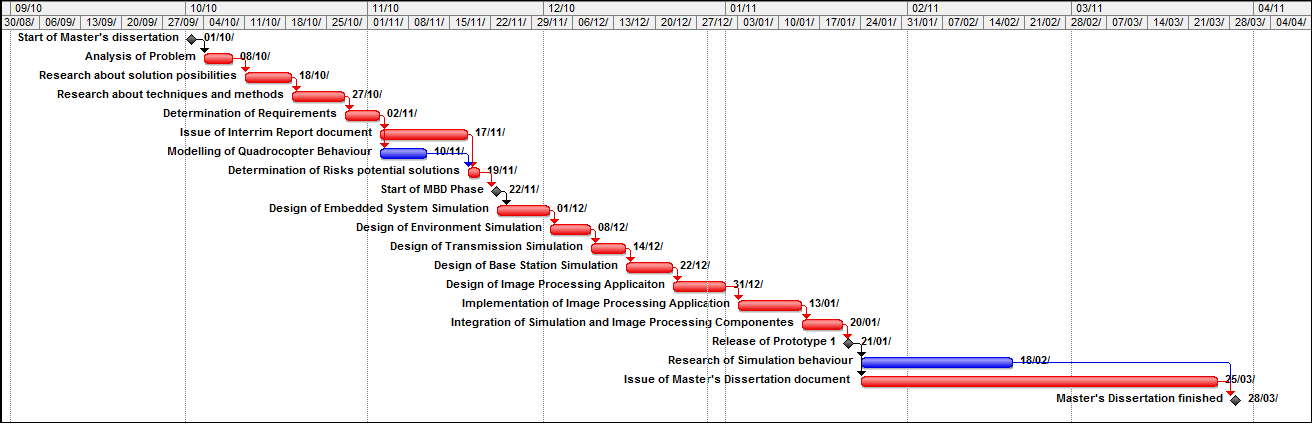
\includegraphics[width=1.1\textwidth, height=180px]{graphic/ProjectPlan.png}
\caption
{The Project Plan}
	\label{fig:ProjectPlan}
\end{figure}
